\documentclass[11pt,letterpaper]{article}
\usepackage[margin=0.88in,headheight=16pt,headsep=18pt]{geometry}
\usepackage[T1]{fontenc}
\usepackage{lmodern,microtype,amsmath,amssymb,amsthm,mathtools,booktabs,array,enumitem,tikz,fancyhdr}
\usepackage[hidelinks,pdftitle={Oracle-Attested Mathematical Knowledge - Completion C - The Epistemic Conservation of Mathematical Histories},pdfauthor={<Brian Tenneson>},pdfsubject={ATLAS-repaired version 0.2: effective reconstruction and a worked oracle-ledger compression}]{hyperref}
\usetikzlibrary{arrows.meta,positioning,calc,fit}
\setlist{nosep,leftmargin=*,topsep=4pt}
\emergencystretch=2em
\pagestyle{fancy}\fancyhf{}
\fancyhead[L]{\small Completion C: Epistemic Conservation}
\fancyhead[R]{\small\texttt{<Brian Tenneson>}}
\fancyfoot[C]{\thepage}
\newtheorem{theorem}{Theorem}[section]
\newtheorem{lemma}[theorem]{Lemma}
\newtheorem{proposition}[theorem]{Proposition}
\newtheorem{corollary}[theorem]{Corollary}
\theoremstyle{definition}
\newtheorem{definition}[theorem]{Definition}
\newtheorem{example}[theorem]{Example}
\newtheorem{remark}[theorem]{Remark}
\newtheorem{conjecture}[theorem]{Conjecture}
\newcommand{\N}{\mathbb N}
\newcommand{\Hh}{\mathcal H}
\newcommand{\Obs}{\mathcal O}
\newcommand{\Act}{\mathcal A}
\newcommand{\State}{\mathcal S}
\newcommand{\Ph}{\Phi}
\newcommand{\Cert}{\mathsf{Cert}}
\newcommand{\Att}{\mathsf{Att}}
\newcommand{\Rel}{\mathsf{Relay}}
\newcommand{\Tr}{\mathsf{Trusted}}
\newcommand{\Adm}{\mathsf{Adm}}
\newcommand{\View}{\mathsf{View}}
\newcommand{\pre}{\preceq}
\newcommand{\defined}{\mathord\downarrow}
\title{\bfseries Oracle-Attested Mathematical Knowledge\\[3pt]
\large Completion C: The Epistemic Conservation of\\ Mathematical Histories\\[3pt]
\normalsize Exact Audit Preservation, Indistinguishability, and the Memory Needed for Continuing Verification}
\author{\texttt{<Brian Tenneson>}\\\small Mathematical development and manuscript preparation assisted by DATA MIND (OpenAI GPT-6)}
\date{October 30, 2026\\\small ATLAS-repaired version 0.2; successor to FDWC Level-1 Completions A and B; sources unchanged}
\begin{document}
\maketitle
\begin{center}
\small\bfseries See the disclaimer on mathematical accuracy, authorship, and artificial intelligence following this essay.
\end{center}
\begin{abstract}
A typed evidence calculus can preserve proof and oracle-testimony records after a truth source disappears; indistinguishability arguments also show that erased distinctions cannot in general be reconstructed. We combine these directions into a new audit-preservation problem: exactly which distinctions between finite histories must a Pioneer retain to answer an authorized collection of epistemic questions? For a fixed finite-ledger audit interface $Q$ and retention map $R$, we prove that exact retrospective reconstruction is possible precisely when $R$ never identifies histories with different audit outputs. We characterize the coarsest sufficient observational quotient, give an information lower bound for fixed-length archives, and exhibit both an oracle-truth counterexample to effective decoding and an explicit restricted oracle-ledger compression scheme. We then distinguish retrospective preservation from continuation under future events: a retained state supports exact deterministic future updates precisely when its induced equivalence respects observations, enabled actions, and successor states. A coarsest future-observational equivalence exists, but need not be decidable, even when individual observations and transitions are computable. Our example compresses an unbounded family of restricted ledger records into finite state under a declared narrow audit and action alphabet; it makes no claim about full-ledger compression. The results are mathematical constructions relative to declared protocol and effectiveness assumptions; they neither implement a halting oracle nor certify a running AMLD+0 engine.
\end{abstract}
\noindent\textbf{Status and scope.} New conditional theorems are proved at the paper level. No independent proof assistant, external mathematical referee, or running AMLD+0 federation has checked this manuscript. The original proof BANK, policies, and engines are not changed. No optimal physical compression, globally optimal FDWC completion, or unconditional oracle delivery guarantee is claimed. The repaired version distinguishes existential decoding from computable decoding throughout.
\tableofcontents

\section{From two completions to a third problem}
The immutable ancestor $W_0$ asks whether the Pioneer $P^*$ can retain an exact account of proof, oracle testimony, and relay delivery after an ideal truth source $O_T$ is deactivated. The blind relay $O_R$ forwards finite bytes without deciding their truth. Completion A developed the typed, finite-ledger calculus and its verifier firewall; Completion B made the receiver's evidence view explicit and tested reconstruction claims by indistinguishable-history countermodels. Both establish conditional preservation results and both leave audit-preserving compression open.

The present paper takes their interaction, rather than their union, as its subject. Given an authorized family of queries about a finite history, what can the Pioneer discard while retaining \emph{exactly} the answers to those queries? And when the Pioneer must continue processing events, what stronger preservation condition is necessary? These are different questions. A retrospective archive can be correct today but insufficient to validate tomorrow's message. Even a mathematically well-defined decoder may be noncomputable; both distinctions will be witnessed by explicit examples.

\begin{figure}[htbp]\centering
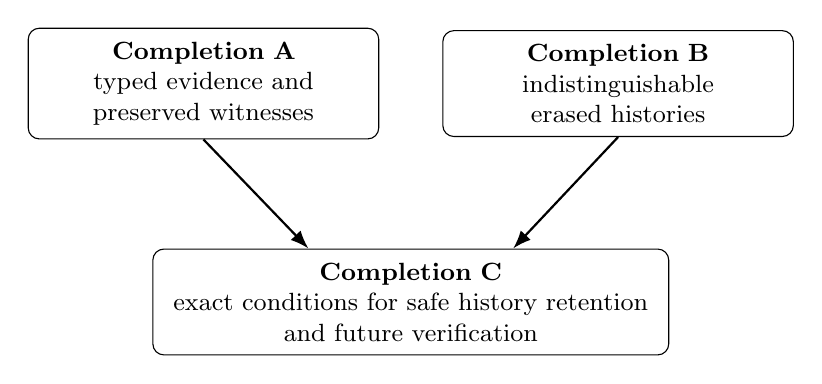
\begin{tikzpicture}[>=Latex, node distance=7mm, every node/.style={font=\small}, box/.style={draw,rounded corners,align=center,minimum height=11mm,inner sep=5pt}]
\node[box,text width=4.1cm] (a) {\textbf{Completion A}\\typed evidence and preserved witnesses};
\node[box,right=8mm of a,text width=4.1cm] (b) {\textbf{Completion B}\\indistinguishable erased histories};
\coordinate (mid) at ($(a.south)!0.5!(b.south)$);
\node[box,below=14mm of mid,text width=6.2cm] (c) {\textbf{Completion C}\\exact conditions for safe history retention\\and future verification};
\draw[->,thick] (a.south) -- ([xshift=-13mm]c.north);
\draw[->,thick] (b.south) -- ([xshift=13mm]c.north);
\end{tikzpicture}
\caption{The synthesis: A supplies the evidence objects; B supplies the indistinguishability obstruction; C asks for exact preservation criteria.}
\label{fig:synergy}
\end{figure}

\paragraph{Interpretive boundary.} An accepted statement, a true statement, and a formally certified statement remain distinct. In particular, the words ``knowledge'' and ``conservation'' below name preservation of a specified \emph{audit interface}; they do not assert unrestricted philosophical knowledge or conservation of all truth. We work entirely from the supplied $W_0$-derived Completions A and B, without adding external mathematical sources.

\section{Frozen protocol and the audit interface}
Fix the inherited environment
\[
M=(\Gamma,F,V,O_T,O_R,P^*,A,\tau,L,c),
\]
where $F$ and $\Gamma$ are the fixed proof calculus and hypotheses; $V$ is a total decidable finite-proof verifier; $A$ is a fixed total decidable authentication, scope, and ancestry policy; $\tau$ is a fixed decidable trust policy; $L$ is a typed append-only finite event ledger at each finite time; and $c$ assigns finite nonnegative rational event charges. The original BANK is immutable and distinct from the proof-event ledger. Only a successful check by $V$ permits proof-event admission. The ideal source answers $H(e)$ correctly by semantic stipulation; that stipulation is not a computable implementation.

\begin{definition}[Admissible finite history]
For this paper a \emph{history} $h$ is a finite, locally closed accepted snapshot, including its finite registered-formula roster, complete accessible payloads and proof objects, finite acyclic ancestry chains, validation data, and the versions and locally executable inputs for $V,A,\tau$. Let $\Hh$ be a stated family of such histories within one fixed protocol profile. Unless otherwise specified, $\Hh$ is the family of syntactically admissible histories under the fixed local acceptance rules; it does \emph{not} require a decision procedure for semantic truth of all oracle assertions. A subclass $\Hh_{\rm true}$ may additionally satisfy the ideal source-truth contract.
\end{definition}

The receiver does not infer unrecorded physical events from a locally closed snapshot. In particular, a pointer whose target disappears with $O_T$ does not constitute a closed witness. The distinction between syntactic acceptance and semantic truth is necessary to avoid silently assuming a halting decider when reasoning about finite records.

\begin{definition}[Typed evidence view]
For each registered effectively encoded sentence $\varphi$, define
\begin{align*}
E_h(\varphi)&=(p_h(\varphi),a_h(\varphi),r_h(\varphi),u(\varphi))\in\{0,1\}^4,\\
p_h(\varphi)&=1\ \Longleftrightarrow\ \exists\pi\text{ in the proof ledger with }V(\pi,\Gamma,\varphi)=1,\\
a_h(\varphi)&=1\ \Longleftrightarrow\ \exists\text{ accepted origin receipt asserting }\varphi,\\
r_h(\varphi)&=1\ \Longleftrightarrow\ \exists\text{ accepted }O_T\to O_R\to P^*\text{ chain asserting }\varphi,\\
u(\varphi)&=1\ \Longleftrightarrow\ \Tr_\tau(O_T,\varphi).
\end{align*}
The inherited policy-relative admission bit is
\[
K_h^\tau(\varphi)=p_h(\varphi)\lor(a_h(\varphi)\land u(\varphi)).
\]
The witness bundle $W_h(\varphi)$ comprises the finite recorded matching proof certificates, origin records, accepted relay chains, and the applicable trust-policy entry. Transport alone cannot add a verified proof. As in A and B, the relay flag is displayed separately rather than being made an extra conjunct in the frozen admission rule.
\end{definition}

\begin{definition}[Authorized retrospective audit]
An \emph{audit interface} $Q:\Hh\to\Obs$ sends each admissible history to a finite, effectively encoded answer to an explicitly stated finite set of questions. The \emph{full finite-roster audit} $Q_{\rm full}$ serializes, in a fixed canonical order, the registered roster and the pairs
\[
\bigl(E_h(\varphi),W_h(\varphi)\bigr)
\quad\text{for each registered }\varphi.
\]
Canonical ordering and finite encodings are fixed in advance. Where witness equivalence rather than byte-for-byte identity is intended, it must be a declared, decidable equivalence with an effective canonical representative for each encountered finite witness object. The corresponding $Q$ records those representatives. A \emph{restricted audit}, such as $Q_K$, may ask only for the admission bits on a fixed roster.
\end{definition}

The object $Q_{\rm full}(h)$ is computable from a locally closed finite $h$: scan the finite proof and message projections, invoke total local checkers, enumerate matching finite witnesses, and serialize the result. This is a \emph{finite-record} computation, not a method for resolving the truth of arbitrary arithmetic statements. For comparisons, either use a common fixed roster or include each varying roster in the audit output.

\begin{figure}[htbp]\centering
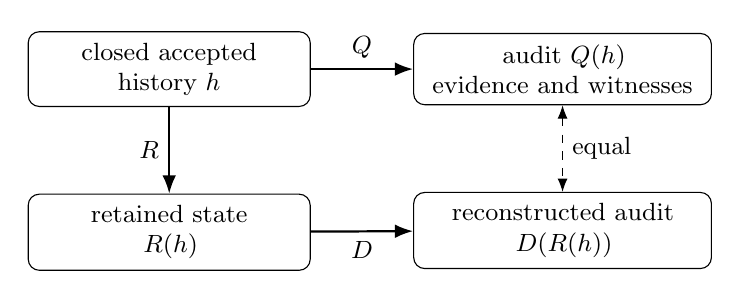
\begin{tikzpicture}[>=Latex,every node/.style={font=\small},b/.style={draw,rounded corners,align=center,minimum height=9mm,inner sep=4pt}]
\node[b,text width=3.3cm] (h) {closed accepted\\history $h$};
\node[b,right=13mm of h,text width=3.5cm] (q) {audit $Q(h)$\\evidence and witnesses};
\draw[->,thick] (h) -- node[above]{$Q$} (q);
\node[b,below=11mm of h,text width=3.3cm] (r) {retained state\\$R(h)$};
\node[b,below=11mm of q,text width=3.5cm] (d) {reconstructed audit\\$D(R(h))$};
\draw[->,thick] (h)--node[left]{$R$}(r);
\draw[->,thick] (r)--node[below]{$D$}(d);
\draw[<->,dashed] (q)--node[right]{equal}(d);
\end{tikzpicture}
\caption{Retrospective sufficiency asks whether the two paths return identical authorized audit answers. It does not require reproduction of every unasked historical fact.}
\label{fig:factor}
\end{figure}

\section{The exact retrospective preservation theorem}
\begin{definition}[Retention and sufficiency]
A \emph{retention map} is a function $R:\Hh\to\State$, where $\State\subseteq\{0,1\}^*$ consists of finite stored representations. It is \emph{$Q$-sufficient} if some reconstruction function $D:R[\Hh]\to\Obs$ satisfies
\[
D(R(h))=Q(h)\quad\text{for every }h\in\Hh.
\]
The requirement is exact equality of authorized audit outputs, not reconstruction of the entire physical execution. No effectiveness or efficiency of $D$ is presupposed in this definition.
\end{definition}

\begin{theorem}[Exact retrospective preservation criterion]\label{thm:static}
A retention map $R$ is $Q$-sufficient if and only if
\begin{equation}\label{eq:kernel}
\forall h_1,h_2\in\Hh,\quad R(h_1)=R(h_2)\ \Longrightarrow\ Q(h_1)=Q(h_2).
\end{equation}
In other words, $\ker(R)\subseteq\ker(Q)$, where $\ker(f)$ denotes equality of outputs under $f$.
\end{theorem}
\begin{proof}
Suppose $Q=D\circ R$. If $R(h_1)=R(h_2)$, applying $D$ to both sides gives $Q(h_1)=Q(h_2)$. Conversely, suppose (\ref{eq:kernel}) holds. For any reachable retained value $s\in R[\Hh]$, choose any $h\in\Hh$ with $R(h)=s$ and set $D(s)=Q(h)$. The hypothesis makes the value independent of the chosen representative. Thus $D$ is a well-defined function on the reachable range and $D(R(h))=Q(h)$ for every $h$.
\end{proof}

The converse is deliberately \emph{extensional}: making $D$ well defined does not, by itself, produce an efficient executable decoder. The following result states a separate sufficient effectiveness condition.

\begin{proposition}[Effective reconstruction on an enumerable domain]\label{prop:effective}
If $\Hh$ has a computable enumeration of its valid finite encodings, $Q$ and $R$ are total computable on those encodings, and (\ref{eq:kernel}) holds, then a partial computable $D$ exists which halts and gives the correct audit on every $s\in R[\Hh]$. No claim is made that membership in $R[\Hh]$ is decidable or that the search is efficient.
\end{proposition}
\begin{proof}
Given $s$, enumerate $h\in\Hh$ until finding one with $R(h)=s$, then output $Q(h)$. Equality of the finite retained encodings is decidable. On every reachable $s$ a preimage eventually appears, so this procedure halts. Equation (\ref{eq:kernel}) makes the result independent of which matching history is first enumerated.
\end{proof}

\begin{remark}[The oracle-truth trap]
Syntactically accepted finite transcripts can be enumerated under a decidable local profile; a family restricted by the requirement that every oracle bit equal the true halting predicate need not be effectively enumerable in the same way. Proposition \ref{prop:effective} is therefore conditional on its stated effective-domain hypothesis, and must not be invoked silently for the oracle-truthful subclass.
\end{remark}


\begin{example}[Extensional sufficiency without any computable decoder]\label{ex:truth-obstruction}
Fix a protocol instance whose decidable syntactic origin policy permits well-formed finite bit receipts. Consider the mathematical family
\[
\Hh_{\rm true}^{\rm bit}=\{h_e=\mathsf{pad}(e,H(e)):e\text{ a standard machine/input code}\},
\]
where $H(e)$ is supplied by the \emph{ideal truthful source}, not computed locally. Here $\mathsf{pad}$ is a fixed computable encoding that embeds an arbitrary finite pair $(e,b)$ in a complete locally closed, syntactically accepted origin-receipt history under this illustrative admissible profile; the other required administrative and checker fields are computably supplied by the fixed profile. This explicitly assumes a profile with a computable syntactic receipt-template constructor, and does not assume that its assertions are semantically true. On the truthful subclass let
\[
R(\mathsf{pad}(e,b))=e,\qquad Q(\mathsf{pad}(e,b))=b.
\]
Both maps are computable projections of the \emph{presented finite records}. Because the truthful family contains exactly one bit for each $e$, $R(h_e)=R(h_f)$ implies $Q(h_e)=Q(h_f)$. Thus Theorem \ref{thm:static} yields a set-theoretic decoder $D(e)=H(e)$. There is nevertheless no ordinary computable decoder on all reachable codes, by the diagonal halting argument. This is not a valid invocation of Proposition \ref{prop:effective}: a computable enumeration of all truthful pairs $(e,H(e))$ would itself compute $H$, by waiting for the enumerated pair with the requested $e$. The example concerns an ideal-source semantic subclass and does not manufacture an executable oracle. In particular, locally closed \emph{stored} original receipts can be audited computably, but deleting the relevant bits destroys this effective guarantee.
\end{example}

\begin{definition}[Effective $Q$-sufficiency]\label{def:effective}
For a stated represented domain, a retention map is \emph{effectively $Q$-sufficient} if an explicitly specified partial computable decoder $D$ halts with $D(R(h))=Q(h)$ on every reachable retained state. A prospective representation is \emph{effectively prospectively sufficient} when its audit decoder, enabled-action test, and retained transition are all partial computable and halt on every permitted reachable input. These are stronger requirements than existence of abstract functions; an algorithm or adequate additional computability hypotheses must be supplied.
\end{definition}

\begin{definition}[Audit equivalence]
Write $h\equiv_Q h'$ if and only if $Q(h)=Q(h')$. Let $[h]_Q$ denote its equivalence class. The quotient map $q_Q:h\mapsto[h]_Q$ is the \emph{canonical observational quotient} associated with the chosen retrospective audit.
\end{definition}

\begin{corollary}[Coarsest sufficient partition]\label{cor:quotient}
The quotient map $q_Q$ is $Q$-sufficient, and every $Q$-sufficient retention map distinguishes at least the pairs distinguished by $q_Q$. Thus $\equiv_Q$ is the coarsest permissible equality-of-retained-state relation for retrospective sufficiency.
\end{corollary}
\begin{proof}
The audit is constant on each $Q$-equivalence class by definition, so Theorem \ref{thm:static} applies to $q_Q$. Any other sufficient $R$ obeys $\ker(R)\subseteq\ker(Q)$ by that theorem.
\end{proof}

This is a mathematical minimality result about \emph{which distinctions must be retained}. It is not a shortest-program theorem, a claim about physical storage optimality, or a unique byte encoding. In a computable finite-record setting $Q(h)$ itself is one canonical sufficient \emph{retrospective} stored output, although computing or maintaining it may be costly and it need not support later updates.

\section{Why admission alone loses epistemic history}
\begin{example}[One admitted proposition, two distinct warrants]\label{ex:proof-vs-att}
Fix a registered sentence $\varphi$ for which $V$ accepts a genuine finite proof from $\Gamma$, and suppose the trusted source can issue an $A$-accepted receipt asserting the same true $\varphi$. A simple instance is a decidably halting machine's correctly encoded halting claim, provided the fixed formal profile admits the indicated proof and receipt. Consider locally closed histories $h_p$ and $h_a$ on the same roster with the same frozen trust flag $u(\varphi)=1$:
\[
\begin{array}{c|cccc|c}
& p&a&r&u&K^\tau\\\hline
h_p&1&0&0&1&1\\
h_a&0&1&1&1&1
\end{array}
\]
The first retains a verifier-accepted proof; the second retains an accepted trusted source receipt and two-hop path, but no proof. Both are admitted under the inherited rule, so $Q_K(h_p)=Q_K(h_a)$ for the one-sentence admission-only audit. However, $Q_{\rm full}(h_p)\ne Q_{\rm full}(h_a)$. A compression that stores only $K^\tau$ is sufficient for the first restricted question and insufficient for the second, richer interface.
\end{example}

\begin{proposition}[Witness sensitivity]\label{prop:witness}
If an audit requires the complete finite accepted witness bundle, then two histories that have the same evidence vector but different required witness encodings cannot be merged by a sufficient retention map. If the audit requires witnesses only up to a declared effective equivalence, it may merge histories whose normalized witness bundles agree.
\end{proposition}
\begin{proof}
In the first case the audit outputs differ because their required witness components differ, so Theorem \ref{thm:static} prohibits equal retention. In the second case normalization makes the respective witness components equal, and there is no obstruction from those components; other audit fields must still agree.
\end{proof}

\begin{remark}[Authenticity is not truth]
These examples distinguish an accepted origin claim from a verified proof without inferring mathematical truth from a signature. A statement admitted via $a\land u$ is sound only if the trusted source assertions are in fact correct; a statement admitted via $p$ requires the intended soundness of $V$ and $\Gamma$. The verifier firewall remains unchanged.
\end{remark}


\section{A worked oracle-ledger compression and a future-action obstruction}\label{sec:worked}
The next construction makes the synergy operational in one deliberately narrow, frozen protocol \emph{instance}. It is a mathematical example of a constrained accepted-ledger family, not a modification to the inherited engine or a claim of universal source-trace compression.

\begin{example}[A two-bit continuing archive for an unbounded ledger family]\label{ex:concrete-ledger}
Fix a decidable authentication/ancestry policy $A$, fixed trust policy $\tau$, and the unchanged verifier gate $V$ satisfying the inherited type separation. Choose a true, registered halting-bit sentence $\varphi\equiv H(e_*)=1$, where $e_*$ is a specified immediately halting code, with $\tau$ trusting the source for $\varphi$. Fix two distinct, accepted, source-authenticated receipt templates $r_0,r_1$ asserting $\varphi$, with distinct query identifiers $q_0,q_1$ and complete finite validation data. The templates may be generated by a finite lookup table; their acceptance is part of the stated finite instance of the frozen profile. Also choose an unrelated true sentence $\psi\equiv H(e_\infty)=0$ for an explicitly looping machine, and permit an arbitrary finite number $n$ of distinct, locally closed, source-authenticated $\psi$-records, none addressed by the actions below. Only finitely many ideal truthful oracle answers (issued before any source deactivation) are used; no local algorithm is required to solve halting. This illustration allows multiple original queries, while the inherited basic preservation theorem needs only one.

For $i,t\in\{0,1\}$ and $n\in\N$, let $h_{i,n,t}$ be a finite locally closed accepted ledger with exactly one $\varphi$-origin record $r_i$, those $n$ auxiliary $\psi$-records, no accepted $\varphi$-proof, and (if $t=1$) exactly one correctly validated two-hop relay chain for $r_i$. If $t=0$, there is no completed $\varphi$-path. All ancestor bytes, independent checker data, and fixed policy versions required for these records remain locally available. The restricted audit asks \emph{only} for the four evidence bits of $\varphi$, not costs, message counts, $\psi$-witnesses, or full provenance:
\[
Q_{\varphi}(h_{i,n,t})=(p,a,r,u)=(0,1,t,1),
\qquad K^\tau(\varphi)=1.
\]
There are infinitely many distinct ledgers because the $\psi$-records have distinct finite identifiers, but the authorized audit has only two outputs. The one-bit retrospective retention
\[
R_{\rm now}(h_{i,n,t})=t,\qquad D_{\rm now}(t)=(0,1,t,1)
\]
is explicitly computable and $Q_{\varphi}$-sufficient, uniformly in $n$.

To model a continuing Pioneer, restrict the action alphabet to $\{\mathsf{deliver}(0),\mathsf{deliver}(1)\}$. The action $\mathsf{deliver}(j)$ is enabled \emph{exactly} when $t=0$ and $i=j$; it appends the correctly authenticated two-hop chain referencing $r_j$ and changes $t$ to $1$. No actions are enabled once $t=1$. The authorization and predecessor checks use the same fixed $A$ and the stored templates; the only supplied new object is the corresponding finite relay envelope. These are the \emph{declared} admissible future actions for this example, not every possible action of a general AMLD ledger.

Define a two-bit archive and explicit transition operations by
\[
R_{\rm cont}(h_{i,n,t})=(i,t),\quad D_{\rm cont}(i,t)=(0,1,t,1),
\]
\[
\mathsf{enabled}((i,t),\mathsf{deliver}(j))\iff (t=0\ \wedge\ i=j),
\]
\[
\bar\delta((i,0),\mathsf{deliver}(i))=(i,1).
\]
These finite algorithms exactly reproduce the audit, enabled actions, and successor retention for the entire family. They discard the unbounded number of auxiliary $\psi$-records and their histories. Thus they give an explicit, nontrivial, \emph{effectively prospectively sufficient} compression for this restricted interface and action set, without changing the proof BANK or allowing a message to enter the proof ledger.
\end{example}

\begin{proposition}[A retained admission or relay flag is insufficient for continuation]\label{prop:concrete-obstruction}
In Example \ref{ex:concrete-ledger}, $R_{\rm now}$ is not prospectively sufficient for the stated two-action transition system. The two-bit map $R_{\rm cont}$ is effectively prospectively sufficient, although it is not claimed to be the coarsest possible encoding.
\end{proposition}
\begin{proof}
The two states $h_{0,0,0}$ and $h_{1,0,0}$ have equal current audit and equal $R_{\rm now}$ value $0$, but $\mathsf{deliver}(0)$ is enabled only in the first. Hence the kernel of $R_{\rm now}$ fails the enabled-action condition of a $Q$-congruence. For $R_{\rm cont}$, equal pairs $(i,t)$ have identical audits and enabled actions. Any enabled delivery maps them to pairs $(i,1)$ independent of $n$. The displayed explicit computable decoder and updater therefore satisfy the stronger effective prospective requirement of Definition \ref{def:effective}.
\end{proof}

\begin{remark}[Exact scope of the compression claim]
This is an improvement in retained-state \emph{size} only when the task deliberately excludes ancillary $\psi$ evidence and costs and prohibits future actions addressing those deleted records. The two-bit archive does \emph{not} preserve $Q_{\rm full}$ on a roster containing $\psi$, the complete witness bundle, all historical charges, arbitrary future reference links, or unrestricted revalidation. Such broader audit requirements can force the discarded records to remain. Any implementation must still account for fixed authentication code, template tables, and the cost of reconstructing or supplying a relay envelope; none of these hidden resources is declared free.
\end{remark}

\begin{figure}[htbp]\centering
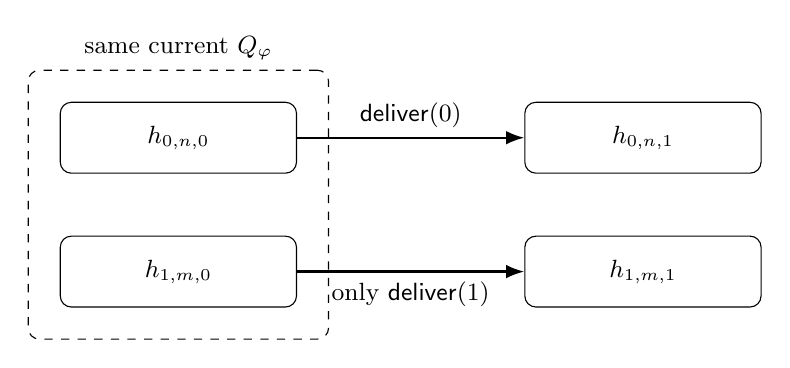
\begin{tikzpicture}[>=Latex, every node/.style={font=\small}, b/.style={draw,rounded corners,align=center,minimum height=9mm,minimum width=30mm,inner sep=4pt}]
\node[b] (a) at (0,0.85) {$h_{0,n,0}$};
\node[b] (b) at (0,-0.85) {$h_{1,m,0}$};
\node[b] (ar) at (5.9,0.85) {$h_{0,n,1}$};
\node[b] (br) at (5.9,-0.85) {$h_{1,m,1}$};
\node[draw,dashed,rounded corners,fit=(a)(b),inner sep=4mm,label=above:{same current $Q_\varphi$}] {};
\draw[->,thick] (a.east)--node[above]{$\mathsf{deliver}(0)$}(ar.west);
\draw[->,thick] (b.east)--node[below]{only $\mathsf{deliver}(1)$}(br.west);
\end{tikzpicture}
\caption{The restricted current audit forgets the receipt ID. A future authenticated predecessor check must still distinguish the two histories. The auxiliary record counts $n,m$ need not survive under this restricted action alphabet.}
\label{fig:worked}
\end{figure}

\section{An information lower bound for finite archival families}
\begin{theorem}[Finite distinguishability bound]\label{thm:bits}
Let $T\subseteq\Hh$ be a nonempty finite family of histories, and put
\[
N=\bigl|\{Q(h):h\in T\}\bigr|.
\]
If $R$ is $Q$-sufficient on $T$, then $\bigl|R[T]\bigr|\ge N$. Consequently, any fixed-length $b$-bit encoding of retained states on $T$ satisfies
\[
b\ \ge\ \left\lceil\log_2 N\right\rceil.
\]
For this \emph{finite specified family} the cardinality bound is achievable by assigning a distinct binary label to each audit-equivalence class; this asserts no uniform or efficient compressor for unbounded history families.
\end{theorem}
\begin{proof}
Choose one history from each of the $N$ distinct audit classes in $T$. By Theorem \ref{thm:static}, no two selected histories can share an $R$-value. Thus at least $N$ distinct retained values are required. There are at most $2^b$ binary strings of length $b$, hence $2^b\ge N$. For attainability on the given finite family, assign distinct labels of length $\lceil\log_2 N\rceil$ to the $N$ classes and use their common audit outputs to define the decoder.
\end{proof}

\begin{example}[Two questions can require more than one flag]
For a one-sentence roster, the restricted interface $Q_K$ has at most two outcomes, so the counting bound alone gives at most one required bit. An interface returning the separate proof, attestation, and relay flags can exhibit more outcomes under a suitable protocol family; each actually realized, distinct evidence pattern contributes another required audit class. Recording the complete witness bundle may yield many more classes even when the Boolean evidence vector is identical.
\end{example}

\paragraph{Cost qualification.} The lower bound measures only the distinguishability of audit outcomes within a fixed finite family. It is not a lower bound on the entire operational memory, on reconstructing all proof or provenance witnesses, or on the minimal time/space needed to maintain a continuing ATP. A coding achieving the bit count may depend on a family-specific lookup table. Variable-length descriptions, expected length under a distribution, storage of checking and decoding code, communication, authentication data, CPU time, and cost charges require separately declared models. The event ledger's finite rational charges make recorded sums computable but do not assign a physical cost to the ideal noncomputable oracle. No optimal compression ratio is claimed.

\section{Continuing agents need more than retrospective sufficiency}
Suppose the Pioneer must process new proof objects, receipts, and relay envelopes after the archive is formed. An answer-preserving snapshot is not necessarily a sufficient \emph{state} for these operations.

\begin{definition}[Deterministic audit transition system]\label{def:trans}
An \emph{audit transition system} is $(\Hh,\Act,\delta,Q)$, where $\Act$ is a specified set of finite action labels and $\delta:\Hh\times\Act\rightharpoonup\Hh$ is a deterministic partial transition map. Definedness means that the action is enabled and its finite accepted successor exists. In an instantiated frozen protocol, actions may represent locally checkable admission or storage steps, with externally supplied payloads named in the action labels. This abstraction neither inserts an oracle query into a computable local transition nor changes the inherited BANK, $V$, $A$, or $\tau$.
\end{definition}

\begin{definition}[$Q$-congruence]
An equivalence relation $\sim$ on $\Hh$ is a \emph{$Q$-congruence} if, whenever $h\sim h'$, (i) $Q(h)=Q(h')$; (ii) for every $a\in\Act$, $\delta(h,a)$ is defined exactly when $\delta(h',a)$ is defined; and (iii) if they are defined, $\delta(h,a)\sim\delta(h',a)$.
\end{definition}

\begin{theorem}[Exact prospective preservation criterion]\label{thm:dynamic}
Let $R:\Hh\to\State$ be a retention map. The following are equivalent:
\begin{enumerate}[label=(\roman*)]
\item There exist well-defined deterministic functions on reachable retained states: a decoder $D$ satisfying $D(R(h))=Q(h)$, an enabled-action predicate agreeing with definedness of $\delta$, and a retained-state successor $\bar\delta$ satisfying $\bar\delta(R(h),a)=R(\delta(h,a))$ whenever the action is enabled.
\item The equivalence relation $\ker(R)$ is a $Q$-congruence.
\end{enumerate}
Consequently, under these conditions the quotient system produces the same audit outputs after every finite action sequence that is enabled from its starting history.
\end{theorem}
\begin{proof}
Assume (i). Equal retained states have equal decoded observations and the same enabled actions; applying the common retained-state successor to either representation gives equal retained successors. These are precisely the three clauses of a $Q$-congruence. Conversely, assume (ii). On a reachable state $s=R(h)$ set $D(s)=Q(h)$, declare $a$ enabled iff $\delta(h,a)$ is defined, and when enabled set $\bar\delta(s,a)=R(\delta(h,a))$. The congruence clauses make all three assignments independent of the chosen representative. This proves (i). For any finite action sequence, induction on its length shows that enabledness agrees and the retained state after each step is the image under $R$ of the full-history state. Applying $D$ yields identical audit outputs at the end of each enabled prefix.
\end{proof}

\begin{figure}[htbp]\centering
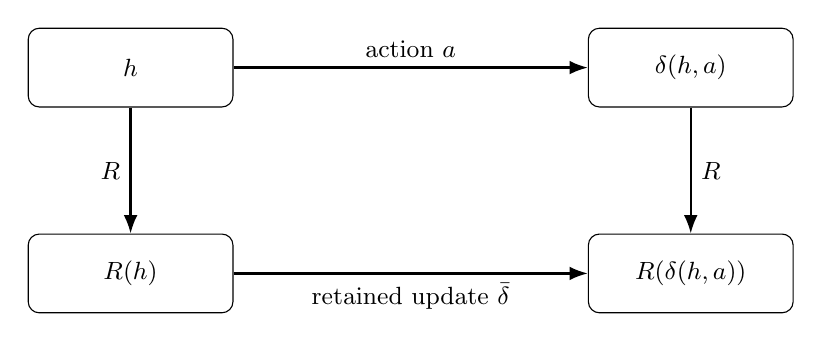
\begin{tikzpicture}[>=Latex,every node/.style={font=\small},b/.style={draw,rounded corners,minimum width=26mm,minimum height=10mm,align=center}]
\node[b] (h) {$h$};
\node[b,right=45mm of h] (ha) {$\delta(h,a)$};
\node[b,below=16mm of h] (rh) {$R(h)$};
\node[b,below=16mm of ha] (rha) {$R(\delta(h,a))$};
\draw[->,thick] (h)--node[above]{action $a$}(ha);
\draw[->,thick] (h)--node[left]{$R$}(rh);
\draw[->,thick] (ha)--node[right]{$R$}(rha);
\draw[->,thick] (rh)--node[below]{retained update $\bar\delta$}(rha);
\end{tikzpicture}
\caption{Prospective preservation requires the retention map to commute with permitted future transitions, not only with today's audit.}
\label{fig:commute}
\end{figure}

\begin{example}[An archive that knows today's answer but cannot process tomorrow's input]
Consider finite histories $x_0,x_1$ with identical current audit output $Q(x_0)=Q(x_1)=0$, and a future action $a$ enabled in both, but with $Q(\delta(x_0,a))=0$ and $Q(\delta(x_1,a))=1$. Retention $R=Q$ is retrospectively sufficient. It is not prospectively sufficient: if $R(x_0)=R(x_1)$, a single deterministic update of that retained state cannot produce both required future answers. In a provenance application, the erased distinction could be validation data needed to judge a subsequently presented predecessor link. This is an abstract countermodel, not an assertion that the frozen A/B protocol implements these four states verbatim.
\end{example}

\begin{corollary}[Verifier-firewall preservation under a suitable audit]
Suppose the authorized audit explicitly includes the verified-proof flags and $\ker(R)$ is a $Q$-congruence for the unchanged protocol transitions. Then every quotient transition has the same displayed proof status as its full-history counterpart. In particular, a message-only transition cannot be represented as increasing the verified-proof flag if it does not do so in the source system.
\end{corollary}
\begin{proof}
By Theorem \ref{thm:dynamic}, the next quotient state decodes to the exact audit of the next full-history state. In the frozen protocol, message-only events leave the proof projection unchanged. Their verified-proof flags therefore remain unchanged in both audited views.
\end{proof}

\section{The coarsest future-observational distinction}
The previous theorem describes safe retained states by a congruence. It is natural to ask whether there is a canonical \emph{largest} such relation, analogous to the retrospective quotient $\equiv_Q$.

For a finite action word $w=a_1\cdots a_n$, let $\delta^*(h,w)$ denote the iterated successor if all actions are enabled, and be undefined otherwise. Put $\delta^*(h,\epsilon)=h$ for the empty word. Let $\bot$ be a fresh symbol not equal to any audit output.
\begin{definition}[Future observational equivalence]
Define
\[
h\equiv_{Q,\delta}^{+}h'
\quad\Longleftrightarrow\quad
\forall w\in\Act^*,\ 
\mathsf{sig}_{h}(w)=\mathsf{sig}_{h'}(w),
\]
where $\mathsf{sig}_h(w)=Q(\delta^*(h,w))$ if the iterated transition is defined, and $\mathsf{sig}_h(w)=\bot$ otherwise.
\end{definition}

\begin{theorem}[Canonical prospective quotient]\label{thm:future}
The relation $\equiv_{Q,\delta}^{+}$ is a $Q$-congruence. Every other $Q$-congruence is contained in it. Thus the quotient by $\equiv_{Q,\delta}^{+}$ is the coarsest \emph{mathematically exact} deterministic retained-state partition preserving every future audit and enabled-action distinction.
\end{theorem}
\begin{proof}
Equality of signatures for all words is an equivalence relation. Taking $w=\epsilon$ proves equality of current $Q$-outputs. For any action $a$, comparing signatures at the one-letter word $a$ proves that $a$ is enabled from both histories or from neither, since $\bot$ is distinct from every audit output. If $a$ is enabled, then for every word $w$ the signature after $a$ followed by $w$ is the signature of successor under $w$. Equality of the original signatures therefore gives $\delta(h,a)\equiv_{Q,\delta}^{+}\delta(h',a)$. Hence it is a congruence.

Conversely, let $\sim$ be any $Q$-congruence and suppose $h\sim h'$. Induction on the length of $w$ shows that either both runs under $w$ are undefined or both are defined with $\sim$-related final states. In the latter case their $Q$-outputs agree. Hence their signatures agree for all words, proving $h\equiv_{Q,\delta}^{+}h'$.
\end{proof}

\begin{corollary}[Retrospective versus prospective classes]
\[
\equiv_{Q,\delta}^{+}\ \subseteq\ \equiv_Q.
\]
The inclusion can be strict: equality of present audit answers need not imply equality under future action sequences.
\end{corollary}
\begin{proof}
The empty-word comparison gives the inclusion. Strictness is witnessed by the preceding example with $x_0,x_1$ and action $a$.
\end{proof}

This supplies a concrete answer to the distinction between an archive and a continuing agent. The coarsest safe \emph{historical} quotient is determined by present audit outputs; the coarsest safe \emph{operational} quotient is determined by all possible future audits. Neither quotient is automatically a physically cheapest representation.

\section{The effectiveness boundary for future memory}
A mathematically defined prospective quotient need not have a terminating general membership test, even when every finite individual audit and transition step is computable. We prove this using an elementary bounded-simulation example; it is not an implementation claim about the original oracle protocol.

\begin{theorem}[Undecidability of prospective equivalence in a computable system]\label{thm:undec}
There exists a deterministic audit transition system with finitely encoded states, a computable $\{0,1\}$-valued audit $Q$, and a total computable transition function for its single action, such that no total computable procedure decides whether two presented states are future-observationally equivalent.
\end{theorem}
\begin{proof}
Let the system have states $s_{e,k}$, for each machine/input code $e$ and $k\in\N$, together with one state $z$. Its only action is $a$, and let
\[
\delta(s_{e,k},a)=s_{e,k+1},\qquad \delta(z,a)=z.
\]
Set $Q(z)=0$ and
\[
Q(s_{e,k})=\begin{cases}
1,&\text{if the machine coded by $e$ halts within $k$ simulated steps},\\
0,&\text{otherwise.}
\end{cases}
\]
The transition and each audit value are computable by finite operations. From $s_{e,0}$, the sequence of audit outputs is identically zero exactly when the machine coded by $e$ never halts (using the standard zero-step convention). Since every audit from $z$ is zero, $s_{e,0}\equiv_{Q,\delta}^{+}z$ if and only if $e$ never halts. A total decision procedure for this equivalence would decide nonhalting and therefore halting on arbitrary inputs, contradicting the standard diagonal halting argument.
\end{proof}

\begin{remark}[What does and does not follow]
Theorem \ref{thm:undec} says a universal algorithm for the coarsest future quotient is impossible across all computable audit transition systems. It does \emph{not} rule out decidable future equivalence for particular finite-state or suitably restricted protocols, and it does not imply that the inherited oracle-ledger model contains this exact abstract subsystem. It shows why an extensional existence theorem must not be advertised as an effective compression algorithm without further structural hypotheses.
\end{remark}

\section{Source deactivation, horizons, and semantic limits}
\begin{proposition}[Closed-history survival: abstract and effective forms]\label{prop:oracle}
Assume the successful source-to-relay handoff, durability, successful post-deactivation delivery, source-independent validation, and locally closed receiver storage stipulated in A and B. Once an admissible receiver history $h$ is installed, a $Q$-sufficient retention $R(h)$ admits a \emph{mathematically defined} reconstruction of the chosen retrospective audit without using a new oracle answer. The Pioneer can \emph{execute} that reconstruction from its retained representation only if the decoder is computable on all required reachable states (for instance, by Proposition \ref{prop:effective} under its enumeration hypotheses, or by an explicit decoder). For an effectively continuing Pioneer, the prospective criterion of Theorem \ref{thm:dynamic} must additionally hold and its induced audit, enabledness, and update operations must be computable as specified in Definition \ref{def:effective}.
\end{proposition}
\begin{proof}
The inherited handoff hypotheses establish a finite locally closed history without a new oracle query. Theorem \ref{thm:static} yields a well-defined set-theoretic decoder on the image of $R$, but the construction by choosing a preimage does not itself give an algorithm. Effectiveness follows only from an additional effective-decoding hypothesis; Example \ref{ex:truth-obstruction} shows why this cannot be omitted for a truthful-oracle family. Theorem \ref{thm:dynamic} separately gives the extensional prospective criterion. Its abstract quotient operations are executable only when there are algorithms for decoding, enabledness, and updates, as the restricted construction in Example \ref{ex:concrete-ledger} demonstrates.
\end{proof}

Both ancestors use the one-drop horizon
\[
h_e(k)=\begin{cases}2,&e\text{ has not halted in its first $k$ simulated steps},\\1,&e\text{ has halted by step $k$},\end{cases}
\]
whose values are computable individually but whose permanent stabilization stage cannot be selected by a total ordinary computable function for every $e$. The predicate
\[
F(e,N)\iff \forall k\ge N\ [h_e(k)=h_e(N)]
\]
has the Turing degree of the halting problem: an $H$-oracle decides whether a future change occurs; conversely, $F(e,0)$ is true exactly when $e$ never halts. The inherited oracle receipt grammar permits only halting-bit assertions. A verified effective reduction from finality to a legitimate halting-bit query supports a separately typed \emph{derived testimonial note}, not a native source attestation of $F(e,N)$ and not a $V$-accepted proof of finality.

\begin{proposition}[Finite preserved answers do not yield universal oracle power]
Any fixed finite, source-deactivated archive of oracle-answer bits can be hard-coded as a finite constant in an otherwise computable procedure. It does not, solely by being preserved or losslessly re-encoded, make that procedure a total decider for the halting predicate on all inputs.
\end{proposition}
\begin{proof}
If a uniform computable algorithm with that fixed finite archive decided halting on all inputs, hard-code the same finite archive into its program. This yields an ordinary total computable halting decider, contradicting the diagonal argument. Exact compression or decompression of a fixed finite archive changes no part of this reasoning.
\end{proof}

The new prospective-undecidability theorem and the inherited one-drop finality theorem have a common conceptual lesson: a finite current observation and a theorem that a final distinction exists do not imply effective recognition of every future distinction. They are not claimed to be the same predicate or to have identical implementations.

\begin{figure}[htbp]\centering
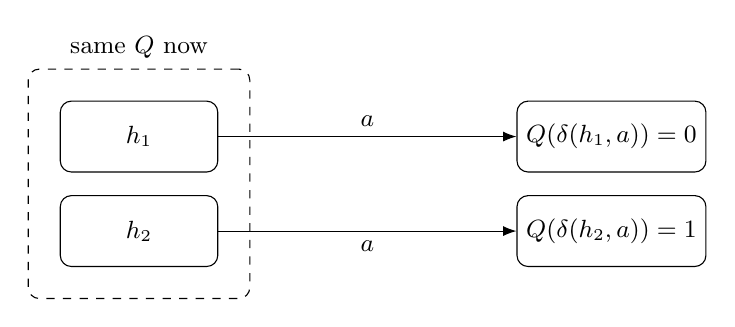
\begin{tikzpicture}[>=Latex,every node/.style={font=\small},b/.style={draw,rounded corners,minimum width=20mm,minimum height=9mm,align=center}]
\node[b] (x) at (0,0.6) {$h_1$};
\node[b] (y) at (0,-0.6) {$h_2$};
\node[draw,dashed,rounded corners,fit=(x)(y),inner sep=4mm,label=above:{same $Q$ now}] {};
\node[b] (xx) at (6,0.6) {$Q(\delta(h_1,a))=0$};
\node[b] (yy) at (6,-0.6) {$Q(\delta(h_2,a))=1$};
\draw[->] (x.east)--node[above]{$a$}(xx.west);
\draw[->] (y.east)--node[below]{$a$}(yy.west);
\end{tikzpicture}
\caption{One current audit class can contain states with different observable futures. Prospective preservation must retain the distinction.}
\label{fig:future-split}
\end{figure}

\section{What Completion C adds, and what remains open}
The synthesis can be stated precisely:
\begin{enumerate}[label=\arabic*.]
\item \textbf{A's constructive side:} authenticated finite evidence, local checker access, source-independent witness persistence, and separation of proof from testimony provide a computable \emph{snapshot audit}.
\item \textbf{B's limiting side:} observationally identical retained states cannot reconstruct different required histories or origins. This becomes the necessary side of the preservation criterion.
\item \textbf{C's additional results:} exact retrospective sufficiency is the kernel-inclusion criterion, but can fail to be computable on a truthful oracle subfamily; a restricted finite-ledger example gives an executable two-bit continuing archive; the canonical retrospective partition is the audit quotient; finite distinguishability yields an archival bit bound; continuing agents require a transition congruence; and the coarsest such prospective equivalence may be undecidable.
\end{enumerate}

From the perspective of discrete writing completion, C is an obligation-directed successor rather than a concatenation of finished texts: A supplies the objects to preserve, B identifies the information-theoretic obstruction, and C resolves their common preservation question under declared hypotheses. This does not yet define a metric on manuscripts, a Cauchy sequence of revisions, a unique completion, or an idempotent completion operator. Such additional structure would be needed before claiming a literal analogue of metric-space completion.

These results are new mathematical propositions \emph{within this paper's development} relative to the two ancestor manuscripts, not independently machine-certified discoveries or claims of absolute novelty against all outside literature. The proof architecture is intentionally modest: small, explicit definitions make the claimed implications independently inspectable.

\begin{conjecture}[Cost-sensitive typed-history compression]
For particular constrained families of finite verifier-gated histories, there may be effectively computable retention schemes that are prospectively sufficient for a nontrivial audit interface and strictly reduce a precisely declared total memory-plus-validation cost relative to storing complete transcripts. No general optimality, strict improvement on every instance, or physical lower bound is asserted without a formal cost model and an explicit construction.
\end{conjecture}

\begin{conjecture}[Useful finite approximations to future equivalence]
For restricted but expressive protocol classes, finite-depth action tests may admit a decidable, monotone refinement procedure whose classes converge extensionally to future-observational equivalence. Such convergence does not in general imply a computable stage at which the true class has been identified.
\end{conjecture}

\paragraph{Candidate Level-2 obligations.} Extend the explicit restricted compression to richer audit interfaces with witness retention and more actions; determine whether the full witness interface or a narrower provenance interface is desired; model resource charges for reconstruction and subsequent validation; investigate source revocation only under a separately authorized time-indexed policy; and give explicit sufficient conditions for decidable prospective equivalence in a suitably restricted frozen protocol. These are future problems, not completed results of C.

\section{Conclusion and verification ledger}
The two Level-1 completions suggest a third question whose answer requires both of their mathematical perspectives. A establishes the kinds of evidence that can survive source loss; B establishes the inability to recover erased distinctions. C characterizes, relative to a specified audit, which distinctions \emph{must} survive. In a static setting, retention is abstractly safe exactly when it refines audit equality; computable reconstruction needs a further effective hypothesis. A concrete restricted oracle-ledger example demonstrates safe two-bit retention for a continuing agent while exhibiting a future check that defeats a one-bit archive. In a continuing setting, safe retention must also preserve enabled actions and the effect of every admissible future step. The resulting future-observational quotient is mathematically canonical but not generally decidable. This distinguishes the existence of an information-preserving abstraction from the ability to compute or cheaply maintain it.

\begin{center}\small
\begin{tabular}{@{}p{0.39\linewidth}p{0.53\linewidth}@{}}\toprule
\textbf{Claim / obligation}&\textbf{Status in this manuscript}\\\midrule
Finite recorded evidence and verifier firewall&Inherited conditional model from A and B; no engine modifications\\
Exact retrospective criterion and quotient&Proofs supplied in Theorem \ref{thm:static} and Corollary \ref{cor:quotient}\\
Extensional vs. effective decoding&Counterexample \ref{ex:truth-obstruction}; Definition \ref{def:effective}; repaired Proposition \ref{prop:oracle}\\
Restricted executable ledger compression&Explicit construction and proof in Example \ref{ex:concrete-ledger} and Proposition \ref{prop:concrete-obstruction}\\
Finite-family bit lower bound&Proof supplied in Theorem \ref{thm:bits}\\
Prospective criterion and canonical relation&Proofs supplied in Theorems \ref{thm:dynamic} and \ref{thm:future}\\
Universal decidability of prospective quotient&Refuted by the computable countermodel, Theorem \ref{thm:undec}\\
General optimal compression / physical cost&Not proved; deliberately left open\\
Independent proof certification / AMLD+0 run&Not performed\\\bottomrule
\end{tabular}
\end{center}

\clearpage
\section*{Provenance and references}\addcontentsline{toc}{section}{Provenance and references}
\noindent\textbf{Source ancestor $W_0$.} \texttt{<Brian Tenneson>}, \emph{Oracle-Attested Mathematical Knowledge: Blind Relays, Source Deactivation, Verifier Gates, and Noncomputable Finality}, research note 0.1, October 29, 2026 (identified in the supplied Level-1 manuscripts as immutable source).\\[4pt]
\textbf{Direct mathematical sources used for C.} \texttt{<Brian Tenneson>}, \emph{Oracle-Attested Mathematical Knowledge: Completion A---A Typed Evidence Calculus for Blind Relays, Source Deactivation, and Noncomputable Finality}, FDWC Level-1, ATLAS-repaired v1.1, October 30, 2026; and \texttt{<Brian Tenneson>}, \emph{Oracle-Attested Mathematical Knowledge: Completion B---An Epistemic Boundary Theorem for Deactivated Sources and Blind Transmission}, FDWC Level-1, ATLAS-repaired v1.1, October 30, 2026. Both supplied PDF and editable LaTeX versions were available for the present development. No source cited in their inherited bibliographies was separately consulted. Neither original document was altered.

\section*{Disclaimer on Mathematical Accuracy, Authorship, and Artificial Intelligence}\addcontentsline{toc}{section}{Disclaimer on Mathematical Accuracy, Authorship, and Artificial Intelligence}
Every reasonable effort has been made to ensure that the mathematical exposition presented herein is factual, correct, logically sound, sufficiently complete in its treatment of relevant facts (not in the technical sense of G\"odelian completeness), and supported by rigorous proofs or, at minimum, not readily susceptible to refutation. Nevertheless, no guarantee of correctness, completeness, consistency, or provability is implied. The authorship and composition of this work involve a combination of human and artificial intelligence. DATA MIND (OpenAI GPT-6), operating under the direction and mathematical research program of \texttt{<Brian Tenneson>}, assisted in developing mathematical statements, organizing proofs, choosing exposition, and preparing the manuscript. The repaired version additionally distinguishes abstract from executable reconstruction and provides one restricted ledger compression instance. Such assistance is not a substitute for independent mathematical verification. Formal proof-assistant checking, independent refereeing, operational AMLD+0 settlement, and physical validation of a noncomputable oracle were not performed. Statements labeled as conjectures remain unproved; all preservation, effectiveness, and soundness conclusions are limited by their expressly stated hypotheses. This draft is not evidence that a computational engine or protocol has been installed or altered, and it carries no authorization to publish without the author's direction.
\end{document}
